\documentclass[11pt]{amsart}

\usepackage{amsmath}
\usepackage[utf8]{inputenc}
\usepackage{physics}
\usepackage{graphicx}
\usepackage{verbatim}

% Letters instead of numbers for subsections
\renewcommand\thesubsection{\Alph{subsection}}

\title[Problem Set 3]{Electrons \\
		\hrulefill \small{ FYS3410: Problem Set 3 } \hrulefill}

\author{Candidate 33}

\date{\today}

\begin{document}

\maketitle

\section{Drude Model}
One of the basic assumptions of the free electron gas (FEG), or Drude model for electrons in solids, is that the mean free path is of the order of the inter-atomic distance. if this  assumption is questionable, it challenges interpretations of all transport properties in terms of FEG, specifically thermal ($\kappa$) and electrical ($\sigma$) conductivities.

The Drude theory makes three assumptions
\begin{enumerate}
\item Electrons have a scattering time $\tau$. The probability of scattering within a time interval $dt$ is $dt/\tau$.
\item Once a scattering event occurs, we assume the electron returns to momentum $\vb{p} = 0$.
\item In between scattering events, the electrons, which are charge $-e$ particles, respond to the externally applied electric field $\vb{E}$ and magnetic field $\vb{B}$.
\end{enumerate}

The failures of the Drude theory:
\begin{itemize}
\item The Hall coefficient frequently is measured to have the wrong sign, indicating a charge carrier with charge opposite to that of the electron.
\item There is no $\frac{3}{2}k_B$ heat capacity per particle measured for electrons in metals. This then makes the Peltier and Seebeck coefficients come out wrong by a factor of $100$.
\end{itemize}

\subsection{Prediction of Wiedemann-Franz}
The most impressive success of the Drude model at the time it was proposed was its explanation of the empirical law of Wiedemann and Franz. 

Firstly, the Lorentz force on an electron is given by
\begin{equation}
\label{eq:lorentz}
\vb{F} = -e(\vb{E} + \vb{v} \times \vb{B})
\end{equation}
Now, consider an electron with momentum $\vb{p}$ at a time $t$. What will the momentum of the electron be at a time $t + dt$? There is a probability $dt/\tau$ that it will scatter to momentum zero. If it does not scatter, it will accelereated as dictated by newtons second law of motion\footnote{$\vb{F} = \frac{d\vb{p}}{dt}$} at probability $1 - dt/\tau$. The expected value of the momentum becomes 
\begin{equation}
\ev{\vb{p}(t + dt)} = \left( 1- \frac{dt}{\tau} \right) (\vb{p}(t) + \vb{F}dt) + \vb{0}\frac{dt}{\tau}.
\end{equation}
This can be rearranged if one keeps the terms in linear order of $dt$
\begin{equation}
\frac{d \ev{\vb{p}}}{dt} = \vb{F} - \frac{\ev{\vb{p}}}{t},
\end{equation}
where $\vb{F}$ is the Lorentz force from equation \ref{eq:lorentz}, of course. Assuming that the electric field is non-zero, the magnetic field is zero, and writing $\ev{\vb{p}}$ as $\vb{p}$ we get
\begin{equation}
\frac{d\vb{p}}{t} = -e\vb{E} -\frac{\vb{p}}{\tau}.
\end{equation}
In a steady state $d\vb{p}/dt= 0$ which gives
\begin{equation}
m\vb{v} = \vb{p} = -e\tau \vb{E} \quad \rightarrow \quad \vb{v} = -\frac{e\vb{E}\tau}{m},
\end{equation}
where $m$ is the mass of the electron and $\vb{v}$ is its velocity.

If there is a density of $n$ of electrons in the metal each with charge $-e$, and they ar all moving at velocity $\vb{v}$, the the electrical current is given by
\begin{equation}
\vb{j} = -en\vb{v} = \frac{e^2\tau n}{m}\vb{E}.
\end{equation}
The electrical conductivity of the metal, defined via $\vb{j} = \sigma\vb{E}$, is given by
\begin{equation}
\label{eq:electricalconductivity}
\sigma = \frac{e^2\tau n}{m}.
\end{equation}

From the kinetic theory of gas we have that the thermal conductivity is
\begin{equation}
\label{eq:kinteticthermal}
\kappa = \frac{1}{3} n C_v \ev{v} \lambda,
\end{equation}
where $\ev{v}$ is the average thermal velocity and  $\lambda = \ev{v} \tau$ is the scattering length. For a monatomic gas the heat capacity per particle is
\begin{equation}
\label{eq:monoheatcap}
C_v = \frac{3}{2}k_B, 
\end{equation}
and 
\begin{equation}
\label{eq:monoavgvel}
\ev{v} = \sqrt{\frac{8k_BT}{\pi m}}.
\end{equation}
Inserting \ref{eq:monoheatcap} and \ref{eq:monoavgvel} into equation \ref{eq:kinteticthermal} yields
\begin{equation}
\kappa = \frac{4}{\pi} \frac{n\tau k_B^2T}{m}.
\end{equation}
While this quantity has the unknown parameter $\tau$ in it, equation \ref{eq:electricalconductivity} contains the same quantity. Thus, we may look at the ratio of thermal conductivity to electrical conductivity,
known as the Lorenz number
\begin{equation}
L = \frac{\kappa}{T\sigma} = \frac{4}{\pi}\left(\frac{k_B}{e} \right)^2.
\end{equation}
A slightly different prediction is obtained by realising that $\ev{v}^2$ was used in this calculation, whereas one can use $\ev{v^2}$ instead\footnote{From kinetic theory: $C_v T = \frac{1}{2}m\ev{v^2}$}. This gives
\begin{equation}
\label{eq:durderesult2}
L = \frac{\kappa}{T\sigma} = \frac{3}{2} \left(\frac{k_B}{e} \right)^2.
\end{equation}

This result was seen as a big success for the Drude model, because it was known for a long time that almost all metals have roughly the same value for this ratio. This fact is called the Wiedemann-Franz law.

\subsection{Free electron Fermi gas}
For a free electron Fermi gas, the heat capacity is given as
\begin{equation}
C_{\text{el}} = \frac{\pi^2}{2} \frac{N k_BT}{T_F}
\end{equation}
and the Fermi velocity is given as
\begin{equation}
v_f = \frac{\hbar k_F}{m},
\end{equation}
where $k_F$ is the Fermi wavevector. This gives a new expression for the heat conductivity
\begin{equation}
\kappa = \frac{\pi^2}{6}\frac{Nnk_BT\hbar^2k_F^2\tau}{T_F m^2},
\end{equation}
while the electrical conductivity ($\sigma$) is the same and given by equation \ref{eq:electricalconductivity}. The Lorenz factor becomes
\begin{equation}
\label{eq:FEFGlorenz1}
L = \frac{\kappa}{T	\sigma} = \frac{\pi^2}{6}\frac{Nk_Bk_F^2\hbar^2}{e^2T_F m},
\end{equation}
which is somewhat of a mess, but replacing the Fermi temperature with
\begin{equation*}
T_F = \frac{E_F}{k_B} = \frac{N\hbar^2k_F^2}{2mk_B}
\end{equation*}
turns the expression in \ref{eq:FEFGlorenz1} into
\begin{equation}
L = \frac{\kappa}{T\sigma} = \frac{\pi^2}{3}\frac{k_B^2}{e^2}.
\end{equation}
This is somewhat similar to what I obtained in equation \ref{eq:durderesult2}.

\begin{comment}
\section{Density of States in Free Electron Fermi Gas}
By introducing Born-Von Karman boundary conditions, one can derive the density of states for a free electron Ferim gas (FEFG) in a three-dimensional sample. Born-von karman means that the wave function is periodic. Here is how such a condition would look like in one dimension:
\begin{equation}
\psi_x(x + L) = \psi_x(x),
\end{equation}
where $L$ is the length (size in one dimension) of the sample. A plane wave solution in three dimensions will satisfy such a periodicity requirement:
\begin{equation}
\psi(\vb{r}) = A\cos(k\vb{r}) + iB\sin(k\vb{r}) \propto e^{ikx}
\end{equation}
where the wavevector is quantised in all dimensional directions such that
\begin{equation*}
k_x = \frac{2\pi}{L}n_x, \text{ for } n_x = 1, 2, 3, \dots
\end{equation*}
By choosing a Hamiltonian without potential, since the electrons are free, the Schrödinger equation gives
\begin{align*}
\hat{H}\psi(\vb{r}) &= E\psi(\vb{r}) \\
-\frac{\hbar^2\nabla}{2m_e}\psi(\vb{r}) &= E\psi(\vb{r}) \\
\rightarrow E &= \frac{\hbar^2 \vb{k}^2}{2m_e}.
\end{align*}

In the ground state of a system of $N$ free electrons, the occupied orbitals may be represented as points inside a sphere in $\vb{k}$ space. The energy on the surface on the sphere is the Fermi energy; the wavevectors at the Fermi surface have a magnitude $k_F$ such that
\begin{equation}
\epsilon_F = \frac{\hbar^2}{2m}k_F^2.
\end{equation}
There will be to electrons per $k$-states because of spin, such that $\text{DOS} = 2\frac{1}{(2\pi/L)^3} = 2\left(\frac{L}{2\pi} \right)^3 = \frac{V}{4\pi^3}$. $k_F$  forms a sphere in $k$-space with volume $V_F = \frac{4\pi}{3}k_F^3$, which contains $N = V_F \times \text{DOS} = \frac{k_F^2}{3}\frac{V}{\pi^2}$ occupied states. Rewriting this gives
\begin{align}
k_F = &\left(\frac{3\pi^2N}{V} \right)^{\frac{1}{3}} \\
\epsilon_F =\frac{\hbar^2}{2m_e} &\left(\frac{3\pi^2N}{V} \right)^{\frac{2}{3}}.
\end{align}
Moreover, the Fermi velocity is found by way of $\epsilon_F = \frac{1}{2}mv_F^2$
\begin{equation}
v_F = \sqrt{\frac{2\epsilon_F}{m}} = \frac{\hbar}{m_e}\left(\frac{3\pi^2 N}{V} \right)^{\frac{1}{3}} = \frac{\hbar k_F}{m_e}.
\end{equation}
Lastly, the Fermi temperature can be found with the relation $k_BT_F = \epsilon_F$
\begin{equation}
T_F = \frac{\hbar^2}{2m_ek_B}\left(\frac{3\pi^2 N}{V} \right)^{\frac{2}{3}}
\end{equation}

EXPLAIN THE TREND!

\end{comment}

\setcounter{section}{2}

\section{Free Electron Fermi Gas}
\subsection{The Chemical Potential at Absolute Zero}
In a one-dimensional sample, the number of electrons will be
\begin{equation}
N_e = 2\int \frac{d \epsilon}{2\pi\hbar /L}f(\epsilon_k)
 = \frac{L}{\pi\hbar} \int d\epsilon \frac{1}{e^{(\frac{k^2}{2m} -\mu)/{k_B T}} + 1},
\end{equation}
dividing by $L$ on both sides give
\begin{equation}
\frac{N_e}{L} = \frac{1}{\pi\hbar} \int d\epsilon \frac{1}{e^{(\frac{k^2}{2m} -\mu)/{k_B T}} + 1}.
\end{equation}
If we know the density of electrons $N_e/L$, one can solve this equation to find $\mu$. In general, $\mu$ depends on $T$ and the electron density.

As the temperature approaches zero, the Fermi-Dirac distribution, $f(\epsilon_k)$ turns into a step function. At low $T$, $(\epsilon-\mu)/(k_B T)$ becomes very large. Depending on the sign of $\epsilon - \mu$
\begin{equation}
\lim_{T \to 0} \frac{\epsilon - \mu}{k_B T} = 
\begin{cases}
	- \infty, \ & \ \epsilon < \mu \\
	+ \infty, \ & \ \epsilon > \mu
\end{cases}
\end{equation}
Therefore,
\begin{equation}
\lim_{T\to 0} f(\epsilon) = \lim_{T\to 0} \frac{1}{e^{(\epsilon -\mu)/(k_B T)} + 1} =
\begin{cases}
	1, \ & \ \epsilon < \mu \\
	0, \ & \ \epsilon > \mu 
\end{cases}
\end{equation}
It is therefore easy to see that the chemical potential $\mu$ plays the role of $\epsilon_F$ here. In other words $\mu = \epsilon_F$ at $T=0$. This result generalises to higher dimensions.

\subsection{FEFG at $T>0K$}

For any $T$ the Fermi-Dirac distribution becomes $\frac{1}{2}$ if $\mu = \epsilon_F$
\begin{equation}
f(\mu) = \frac{1}{e^{(\mu-\mu)/(k_B T) + 1}} = \frac{1}{e^0 + 1} = \frac{1}{2},
\end{equation}
however, this is only an OK approximation for quite high temperatures. This computation begs the question - at what temperatures is the assumption that $\mu = \epsilon$ reasonable?

Figure \ref{fig:fdd1} illustrates this problem nicely. One can see that the Fermi-Dirac function only is a true step function at very low temperatures, and as the temperature increases, the distribution will be more and more flat, approaching $1/2$.

\begin{figure}
\centering
	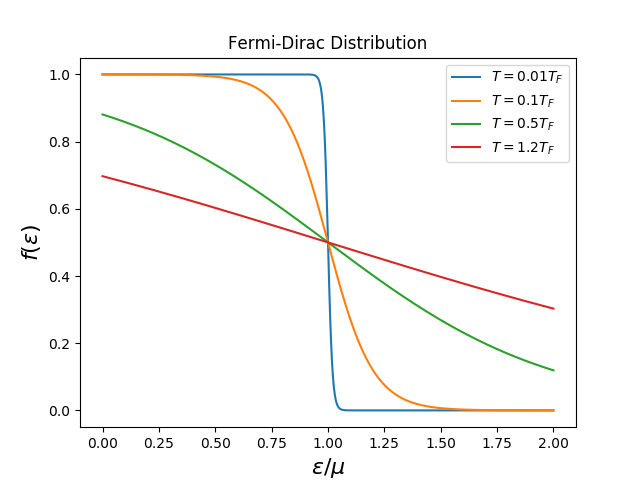
\includegraphics[width = 0.7\textwidth]{fdd1.png}
	\caption{The Fermi-Diract Distribution at different temperatures}
	\label{fig:fdd1}
\end{figure}

\subsection{Chemical Potential Dependence on Temperature}

The total number of orbitals of energy $\leq \epsilon$  in a Fermi sphere is given by
\begin{equation}
N = \frac{V}{3\pi^2}\left(\frac{2m \epsilon}{\hbar^2} \right),
\end{equation}
the same quantity is found by way of the following integral
\begin{equation}
n = \int_0^{\infty} d\epsilon D(\epsilon) f(\epsilon)
\end{equation}

\section{Free Electron Fermi Gas in Lower Dimensions}

\subsection{DOS Independent of Energy in Two Dimensions}
It can be showed that the density of states (DOS) is independent of energy in two dimensions.
\begin{align*}
\text{DOS}_{2D}(k) dk = 2\left(\frac{1}{2} \right)^2\frac{2\pi k}{\frac{\pi}{L_x}\frac{\pi}{L_y}}\frac{1}{V} dk &= \frac{\pi k}{\frac{\pi^2L_xL_yL_z}{L_xL_y}}=\frac{k}{L_z\pi} dk \\
\text{DOS}_{2D}(E) dE &= \text{DOS}_{2D}(k) dk \\
\text{DOS}_{2D}(E) &= \frac{\text{DOS}_{2D}(k)}{\frac{dE}{dk}} \\
				&= \frac{k}{L_z\pi}\frac{2m}{\hbar^2}\frac{1}{2k} \\
				&= \frac{m}{\hbar^2L_z\pi}
\end{align*}

\subsection{DOS Proportional to Inverse Square Root of Energy in One Dimension}
It can be showed that the density of states (DOS) is proportional to $E^{-\frac{1}{2}}$ in one dimension.
\begin{align*}
\text{DOS}_{1D}(k)dk &= 2\frac{1}{2}\frac{1}{\frac{\pi}{L_x}}\frac{1}{V}dk = \frac{1}{\pi}\frac{1}{L_yL_z}dk \\
\text{DOS}_{1D}(E) &= \frac{\text{DOS}_{1D}(k)}{\frac{dE}{dk}} \\
 &=  \frac{1}{\pi}\frac{1}{L_yL_z}\frac{2m}{\hbar^2}\frac{1}{2k} \\
 &= \frac{m}{\hbar^2\pi}\frac{1}{L_yL_z}\frac{1}{k} \\ 
\rightarrow k &= \left(\frac{2m}{\hbar^2}\right)^{\frac{1}{2}} E^{\frac{1}{2}} \\
\text{DOS}_{1D}(E) &= \left(\frac{m}{E} \right)^{\frac{1}{2}} \frac{1}{2\pi\hbar L_y L_z}
\end{align*}

\subsection{DOS Trends for Quantum Wells and Wires}
In quantum wells, the function DOS($E$) has a stair step graph. The wavevector $k = \abs{\vb{k}}$ will lie in a plane with $z$-component equal to $k_{z,1}$ until $(k_x^2+k_y^2)$ is large enough for $k_z$ to be excited. Then the wavevector $k$ is long enough for $k_z$ to be excited from $n_z=1$ to $n_z=2$, for instance. This implies that for energy eigenvalue $E < \frac{\hbar^2}{2m}(k_x^2 + k_y^2 + k_{z,1}^2)$, DOS$_{2D}(E) =0$, and will be increased discretely for higher values of energy $E$.

In one dimension, the wavevector $k$ will only have one degree of freedom. It can only move in one direction, for instance the $x$-direction. The wavevector will increase in magnitude in the $x$-direction until $(k_x^2+k_{y,1}^2+k_{z,1}^2)$ is large enough to excite $k_y$ or $k_z$. At this point DOS$_{1D}(E)$ will jolt upwards and then decrease with $E^{-1/2}$ until again $k_y$ or $k_z$ can be excited.

Figure \ref{fig:dimensionalDOS} provides a good illustration of how the density of states depends on energy, for different dimensionality.

\begin{figure}
\centering
	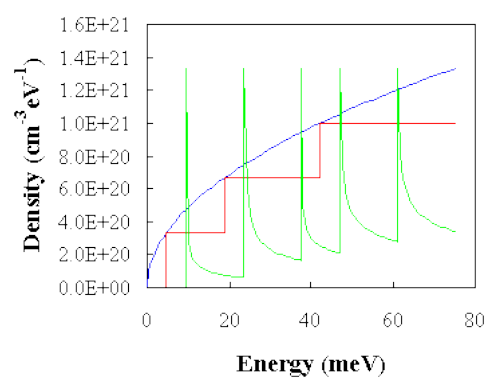
\includegraphics[width=0.7\textwidth]{DOS.png}
	\caption{Density of states as a function of energy for 3D semiconductor (blue curve), a 10nm quantumwell with infinite barriers (red curve) and a 10nm quantum wire with infinite barriers (green curve).}
	\label{fig:dimensionalDOS}
\end{figure}

\subsection{Degeneracy in Quantum Wires}
Assuming that the ``collapsed'' dimensions $y$ and $z$ have the same length, $L=L_y =L_z$, then the expression for energy is simplified to
\begin{equation}
E(n_x, n_y, n_z) = \frac{\hbar^2}{2m}k_x^2 + \frac{\hbar}{2m}\left(\frac{2\pi}{K} \right)^2 (n_y^2 + n_z^2)
\end{equation}
which can be simplified further by concatenating the quantum number in $y$- and $z$-directions, such that $n = n_x + n_y$. In this case, the energy will be the same, independently of $n_y$ and $n_z$, assuming that $n^2 = n_y^2 + n_z^2$ holds. The degeneration will be decided by the number of distributions possible for a particular value of $n^2$. For instance $n^2 = 20$ has degeneracy $2$ because the equation $20 = n_x^2 + n_y^2$ has solutions $(n_x, n_y) = (2, 4)$ and $(n_x, n_y) = (4, 2)$.

\begin{comment}
\section{The Konig-Penney Model}
\begin{figure}
\centering
	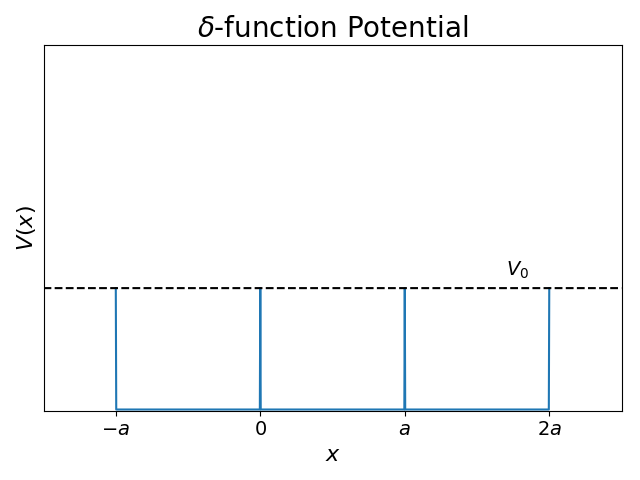
\includegraphics[width=0.7\textwidth]{deltapotential.png}
	\caption{System with potential $V(x) = V_0\delta$, where $\delta$ is $1$ if $x=na$ and $0$ everywhere else.}
	\label{fig:deltapotential}	
\end{figure}

Figure \ref{fig:deltapotential} illustrates a periodic potential of a one-dimensional lattice. The potential has value $V_0$ at atomic sites and is $0$ elsewhere. The wave function in this system would be
\begin{equation}
\psi_{\alpha}(x) = Ae^{ikx} + Be^{-ikx}, \quad k = \sqrt{\frac{2mE}{\hbar^2}}.
\end{equation}
The Bloch theorem states that a general wave function can be expressed as
\begin{equation}
\psi(x) = u(x)e^{iKx}
\end{equation}
where $K$ is a wave vector independent of $k$. Bloch's theorem implies that $\psi(0) = u(0)$ and that $\psi(a) = u(a)e^{iKa}$. Moreover, because $u(a+x) = u(x)$, the ratio
\begin{equation*}
\frac{\psi(a)}{\psi(0)} = \frac{u(a)e^{iKa}}{u(0)} = e^{iKa},
\end{equation*}
gives the relation $\psi(a) = \psi(0)e^{iKa}$, which one may alternatively write as
\begin{align*}
\psi_{\beta}(x) &= \psi_{\alpha}(x-a)e^{iKa}, \\
\psi_{\beta}(x) &= \left[Ae^{ik(x-a)} + Be^{-ik(x-a)} \right]e^{iKa}.
\end{align*}
Since the general wave function $\psi(x)$ must be be continuous then $\psi_{\alpha}(a) = \psi_{\beta}(a)$, which gives
\begin{align*}
\psi_{\alpha}(a) &= \psi_{\beta}(a) \\
Ae^{ika} + Be^{-ika} &= [A + B]e^{iKa} \\
Ae^{ika} + Be^{-ika} &= Ae^{iKa} + Be^{iKa} \\
\end{align*}
\begin{equation}
A \left[e^{iKa} - e^{ika} \right] = B \left[e^{-ika} - e^{iKa} \right].
\end{equation}
Another requirement on the wave function $\psi(x)$ is that its derivative must also be continuous. From the time independent Schrödinger equation (TISE)
\begin{align*}
E\psi(x) &= -\frac{\hbar^2}{2m}\frac{\partial^2}{\partial x^2}\psi(x) + V(x) \psi(x) \\
\rightarrow \frac{\partial^2}{\partial x^2} \psi(x) &= \frac{2m}{\hbar^2}[V(x) - E]\psi(x).
\end{align*}
The first derivative can now be found by way of integration
\begin{equation}
\int_{a-\Delta X}^{a+\Delta x}
\end{equation}

\end{comment}

\setcounter{section}{5}

\section{Monovalent Atom Crystallisation}

\section{Effective Mass}


\end{document}